\documentclass[a4paper,11pt]{article}

% Kódování a jazyk
\usepackage[utf8]{inputenc}
\usepackage[T1]{fontenc}
\usepackage[czech]{babel}
\usepackage{lmodern}

% Matematika
\usepackage{amsmath,amssymb,amsfonts}

% Grafika a layout
\usepackage{graphicx}
\usepackage[margin=2.2cm]{geometry}
\usepackage{float}
\usepackage{booktabs}
\usepackage{array}
\usepackage{multirow}
\usepackage{caption}
\usepackage{subcaption}
\usepackage{enumitem}
\usepackage{fancyhdr}
\usepackage{xcolor}
\usepackage{hyperref}

\hypersetup{
    colorlinks=true,
    linkcolor=blue!60!black,
    citecolor=blue!60!black,
    urlcolor=blue!60!black
}

% Hledání obrázků v podsložkách jednotlivých příkladů
\graphicspath{{1E/}{2E/}{3E/}{4E/}{5E/}}

% Záhlaví
\pagestyle{fancy}
\fancyhf{}
\fancyhead[L]{\small Spolehlivost konstrukcí -- Úlohy E}
\fancyhead[R]{\small Akademický rok 2025/2026}
\fancyfoot[C]{\thepage}
\renewcommand{\headrulewidth}{0.4pt}

% Vlastní příkazy (sjednocené z dílčích projektů)
\newcommand{\unit}[1]{\,\mathrm{#1}}
\newcommand{\E}[1]{\times 10^{#1}}

\captionsetup{font=small}

\begin{document}

\begin{titlepage}
\centering

% --- Logo VUT (volitelné, fallback na text) ---
\IfFileExists{logo/vut.pdf}{%
    \noindent\includegraphics[width=4cm]{logo/vut.pdf}\hfill\strut
}{%
    \IfFileExists{logo/vut.png}{%
        \noindent\includegraphics[width=4cm]{logo/vut.png}\hfill\strut
    }{%
        \noindent{\bfseries\Large VUT FSI}\hfill\strut
    }%
}

\vspace{0.4cm}
\noindent\rule{\textwidth}{0.8pt}

\vspace{1.2cm}

{\large Vysoké učení technické v Brně\par}
{\large Fakulta strojního inženýrství\par}
{\large Ústav mechaniky těles, mechatroniky a biomechaniky\par}

\vfill

{\Huge\bfseries ÚLOHY E\par}
\vspace{0.6cm}
{\Large Souborné řešení příkladů 1E\,--\,5E\par}

\vspace{1.2cm}

{\Large\itshape Spolehlivost konstrukcí\par}

\vfill

{\large\bfseries Členové týmu\par}
\vspace{0.3cm}
{\large
Tomáš Pavlíček\\[2pt]
Tomáš Sláčik\\[2pt]
Vašek Horčic\\[2pt]
Eduard Paclík\par}

\vspace{1.2cm}

{\normalsize Akademický rok 2025/2026\par}

\end{titlepage}

\tableofcontents
\clearpage

\section{Příklad 1E -- Stochastické vyhodnocení vnitřních účinků nosníku}

\vspace{-2mm}

\subsection*{Zadání a výpočtový postup}

Úkolem bylo vykreslit průběhy vnitřních účinků po délce nosníku, tedy normálové síly \(N(x)\), posouvající síly \(T(x)\) a ohybového momentu \(M(x)\). Vnější zatížení bylo uvažováno jako stochastické. Náhodné veličiny byly popsány normálním a lognormálním rozdělením se středními hodnotami podle obr. \ref{fig:zadani} a variačním koeficientem \(v=0{,}1\).

Řešený nosník je znázorněn na obr. \ref{fig:zadani}. Na nosník působí koncentrovaný moment \(M_0\), síla \(F\) a rovnoměrné spojité zatížení \(q\) na převislém úseku.

\begin{figure}[H]
	\centering
	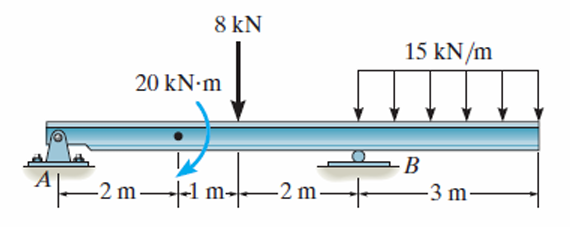
\includegraphics[width=0.92\textwidth,height=0.32\textheight,keepaspectratio]{zadani.png}
	\caption{Schéma zadání.}
	\label{fig:zadani}
\end{figure}

Pro výpočet reakcí bylo spojité zatížení nahrazeno výslednicí

\begin{equation}
	F_q = ql = 15 \cdot 3 = 45\,\mathrm{kN},
\end{equation}

která působí uprostřed zatíženého úseku, tedy v poloze \(x_q = 6{,}5\,\mathrm{m}\). Ze statických rovnic rovnováhy byly určeny reakce ve vazbách

\begin{equation}
	R_B = \frac{3F+19{,}5q+M_0}{5},
	\qquad
	R_A = F+3q-R_B.
\end{equation}

Pro střední hodnoty zatížení vychází

\begin{equation}
	R_A=-14{,}3\,\mathrm{kN}, \qquad
	R_B=67{,}3\,\mathrm{kN}, \qquad
	\max |M| = 67{,}5\,\mathrm{kN\,m}.
\end{equation}

\subsection*{Stochastické vyhodnocení}

Zatížení \(F\), \(q\) a \(M_0\) byla dále uvažována jako náhodné veličiny. Směrodatná odchylka jednotlivých veličin byla určena pomocí variačního koeficientu

\begin{equation}
	\sigma_X = v\mu_X,
	\qquad
	v=0{,}1.
\end{equation}

Výpočet byl proveden metodou Monte Carlo pro \(n = 1\,000\,000\) simulací. V každé simulaci byly vygenerovány náhodné hodnoty zatížení, ze kterých byly vypočteny reakce a průběhy vnitřních účinků. Byly porovnány dvě varianty rozdělení: normální a lognormální. Normální rozdělení je symetrické kolem střední hodnoty, zatímco lognormální rozdělení připouští pouze kladné hodnoty.

\begin{figure}[H]
	\centering
	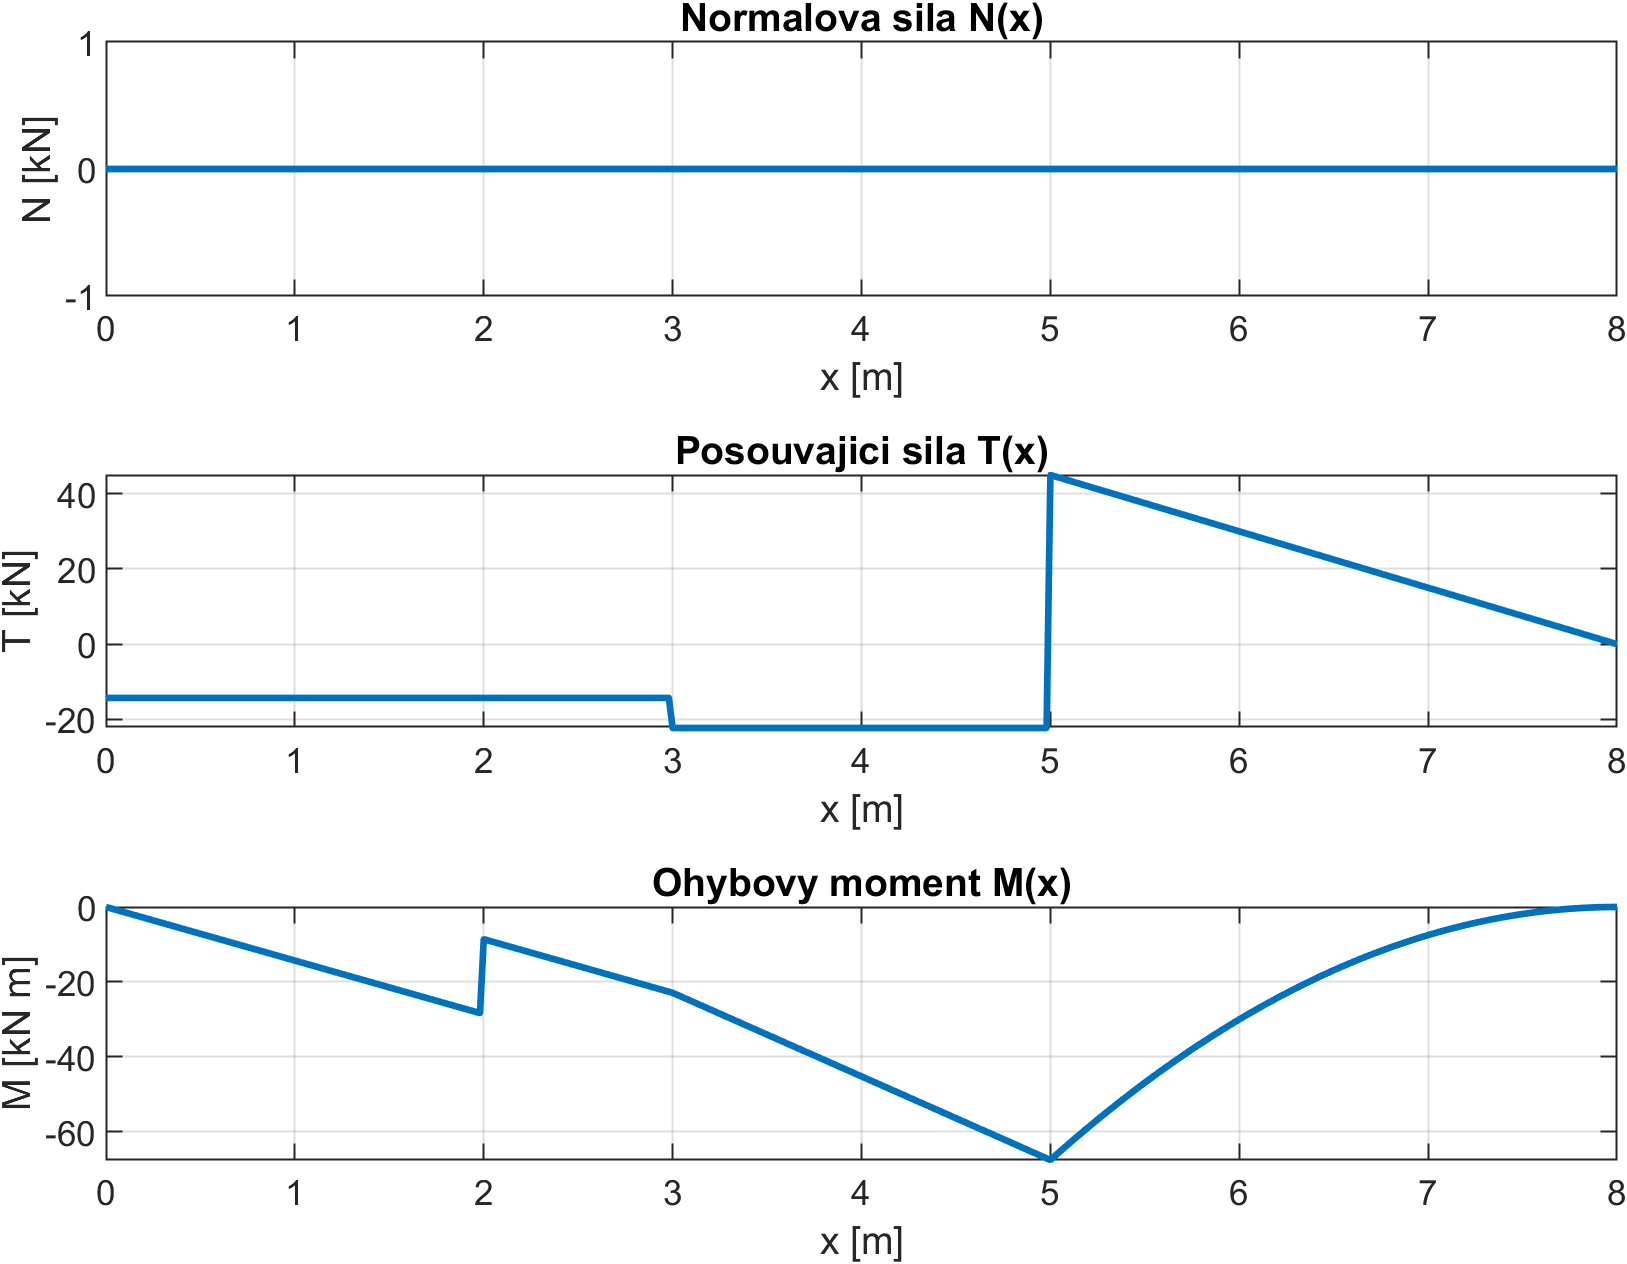
\includegraphics[width=0.82\textwidth,height=0.30\textheight,keepaspectratio]{01_deterministicke_prubehy.png}
	\caption{Deterministické průběhy \(N(x)\), \(T(x)\) a \(M(x)\) pro střední hodnoty zatížení.}
	\label{fig:det}
\end{figure}

\subsection*{Výsledky}

Na obr. \ref{fig:det} jsou uvedeny deterministické průběhy vnitřních účinků. Normálová síla je po celé délce nosníku nulová, protože na nosník nepůsobí vodorovné zatížení. Posouvající síla \(T(x)\) má skoky v místech bodových účinků a na převislé části lineárně klesá vlivem spojitého zatížení. Ohybový moment \(M(x)\) má v místě koncentrovaného momentu skok a na převislé části parabolický průběh.

\begin{table}[H]
	\centering
	\caption{Statistické výsledky pro \(1\,000\,000\) simulací.}
	\label{tab:vysledky}
	\scriptsize
	\begin{tabular}{llrrrr}
		\toprule
		\textbf{Rozdělení} & \textbf{Veličina} & \textbf{Průměr} & \textbf{Směr. odch.} & \textbf{P05} & \textbf{P95} \\
		\midrule
		Normální
		& \(R_A\,[\mathrm{kN}]\) & \(-14{,}298\) & \(1{,}4451\) & \(-16{,}673\) & \(-11{,}922\) \\
		& \(R_B\,[\mathrm{kN}]\) & \(67{,}294\) & \(5{,}8869\) & \(57{,}613\) & \(76{,}978\) \\
		& \(\max |M|\,[\mathrm{kN\,m}]\) & \(67{,}492\) & \(6{,}7547\) & \(56{,}388\) & \(78{,}604\) \\
		\midrule
		Lognormální
		& \(R_A\,[\mathrm{kN}]\) & \(-14{,}302\) & \(1{,}4452\) & \(-16{,}774\) & \(-12{,}027\) \\
		& \(R_B\,[\mathrm{kN}]\) & \(67{,}307\) & \(5{,}8852\) & \(58{,}136\) & \(77{,}446\) \\
		& \(\max |M|\,[\mathrm{kN\,m}]\) & \(67{,}507\) & \(6{,}7530\) & \(56{,}989\) & \(79{,}151\) \\
		\bottomrule
	\end{tabular}
\end{table}

Hodnoty P05 a P95 představují 5\% a 95\% percentil. Mezi těmito mezemi se nachází přibližně 90~\% simulovaných výsledků. Tyto hodnoty proto vyjadřují interval, ve kterém se nachází většina výsledků, a současně popisují jejich rozptyl způsobený náhodností zatížení.

\begin{figure}[H]
	\centering
	
	\begin{minipage}[t]{0.49\textwidth}
		\centering
		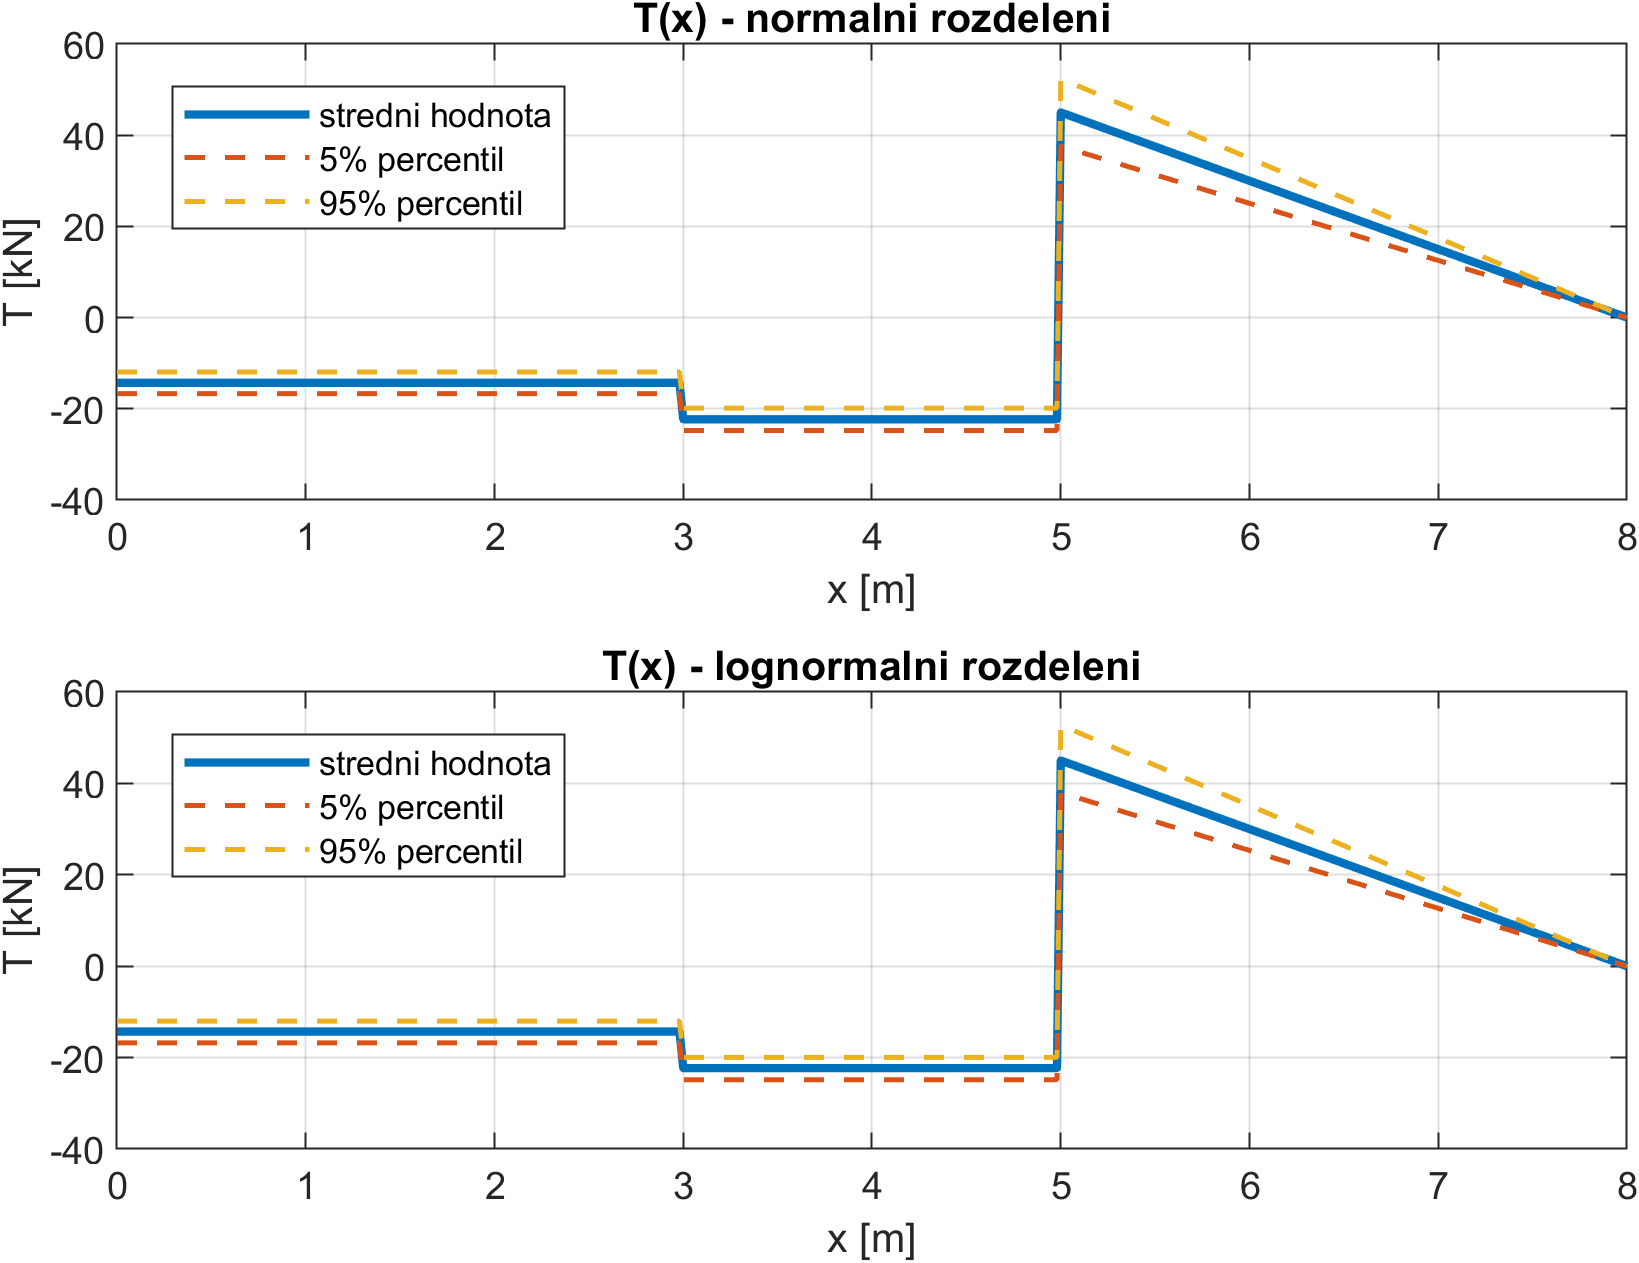
\includegraphics[width=\textwidth,height=0.30\textheight,keepaspectratio]{02_stochasticky_prubeh_T.png}
		{\small (a) Posouvající síla \(T(x)\)}
	\end{minipage}
	\hfill
	\begin{minipage}[t]{0.49\textwidth}
		\centering
		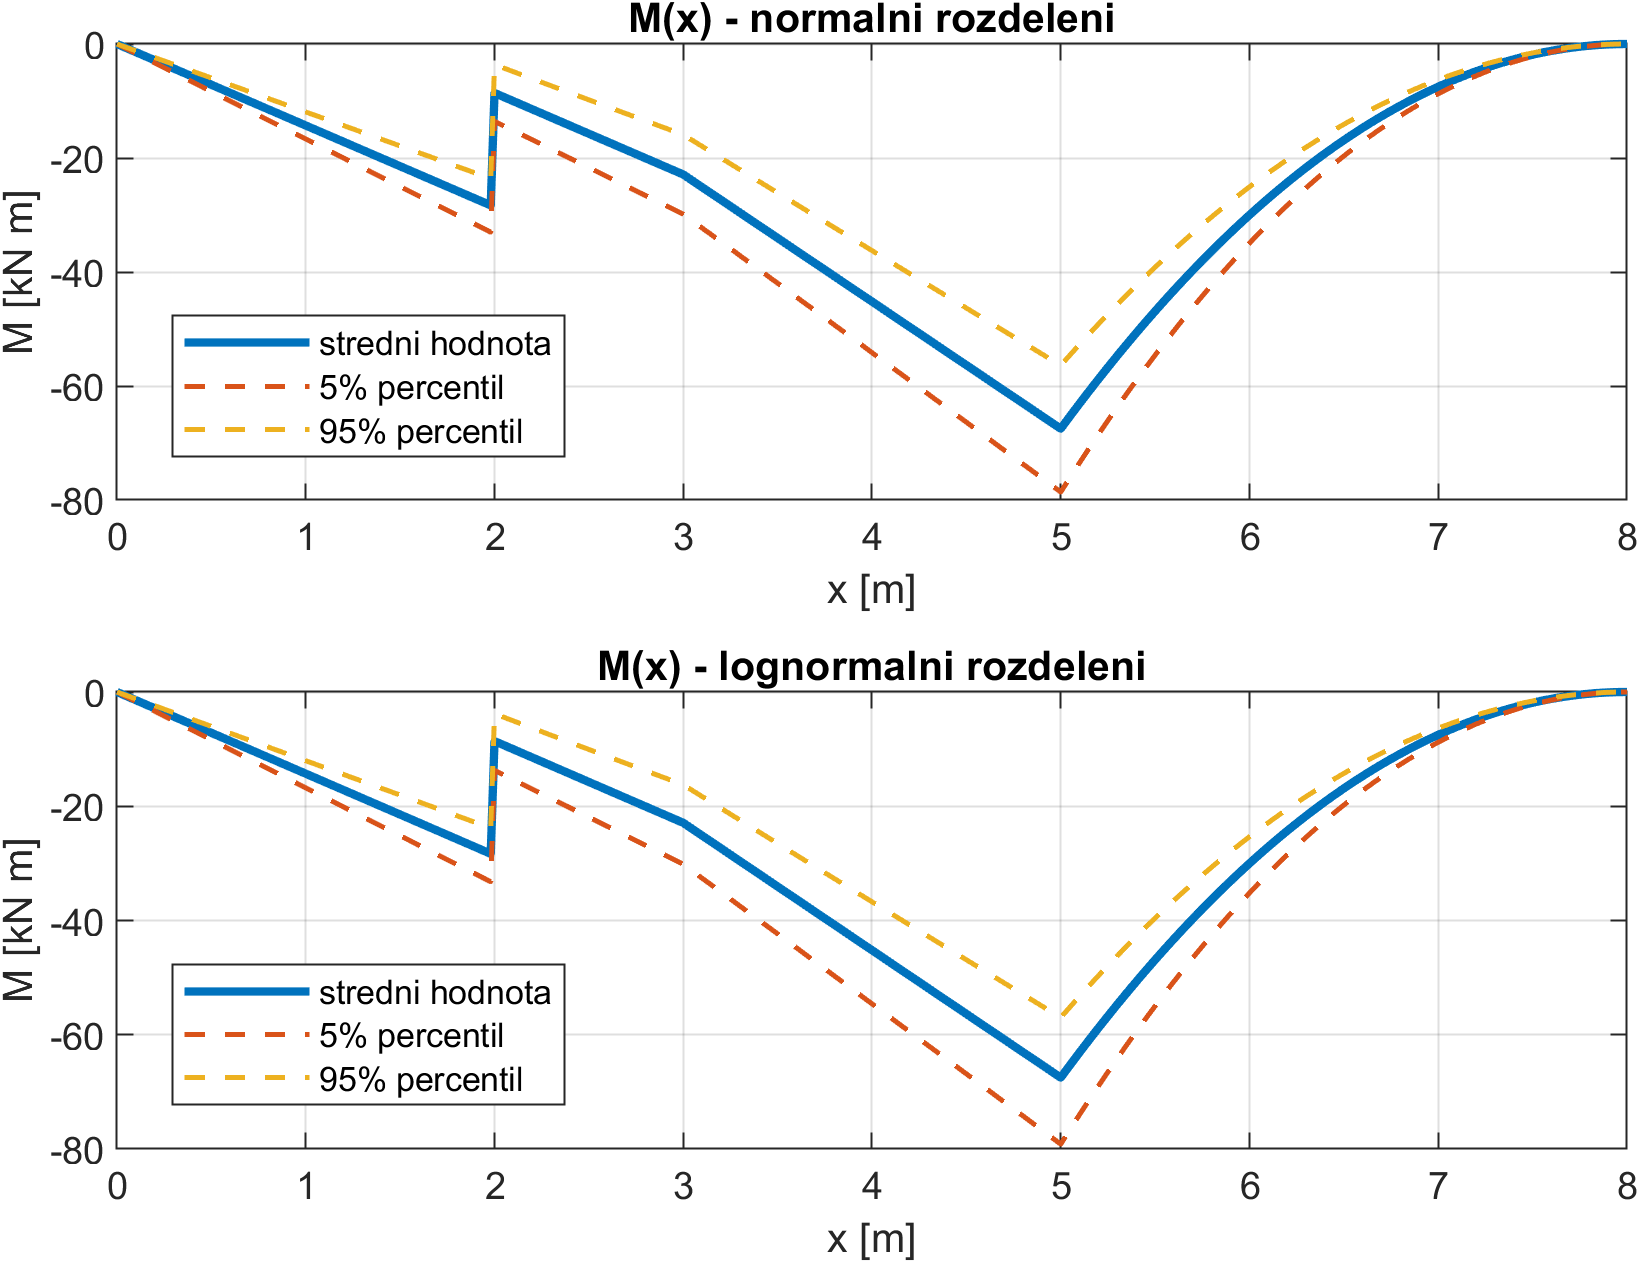
\includegraphics[width=\textwidth,height=0.30\textheight,keepaspectratio]{03_stochasticky_prubeh_M.png}
		{\small (b) Ohybový moment \(M(x)\)}
	\end{minipage}
	
	\caption{Stochastické průběhy posouvající síly \(T(x)\) a ohybového momentu \(M(x)\). Plná čára představuje střední hodnotu, přerušované čáry odpovídají 5\% a 95\% percentilu.}
	\label{fig:stochasticke_prubehy}
\end{figure}

Obr. \ref{fig:stochasticke_prubehy} ukazuje střední průběhy vnitřních účinků a jejich percentilové meze. Šířka percentilového pásma vyjadřuje, jak výrazně se mohou průběhy \(T(x)\) a \(M(x)\) měnit vlivem náhodnosti zatížení. V místech, kde se percentilové křivky sbíhají, je výsledek určen okrajovou podmínkou nebo rovnováhou.

\begin{figure}[H]
	\centering
	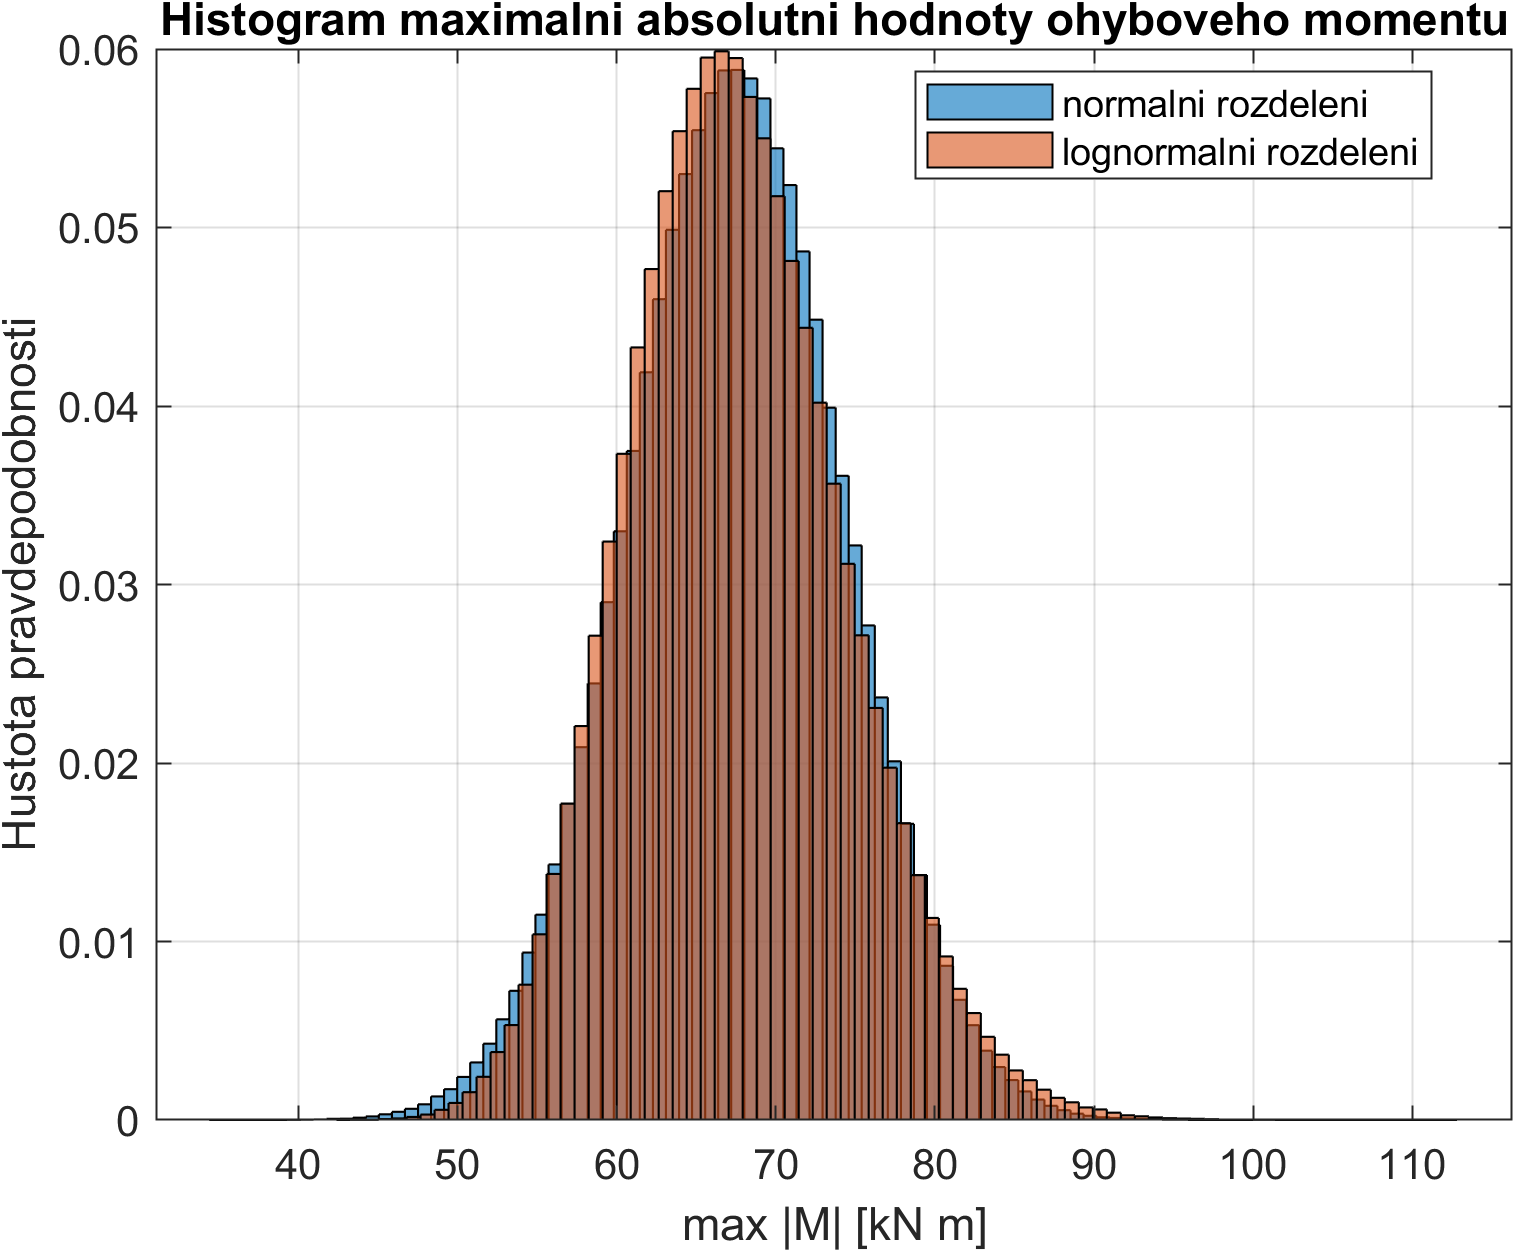
\includegraphics[width=0.92\textwidth,height=0.32\textheight,keepaspectratio]{04_histogram_max_abs_M.png}
	\caption{Histogram maximální absolutní hodnoty ohybového momentu \(\max |M|\) pro normální a lognormální rozdělení zatížení.}
	\label{fig:hist}
\end{figure}

Na obr. \ref{fig:hist} je uveden histogram maximální absolutní hodnoty ohybového momentu. Histogram ukazuje, jak často se v simulacích vyskytovaly jednotlivé hodnoty \(\max |M|\), a doplňuje tak percentilové vyhodnocení o pravděpodobnostní rozdělení maximálního ohybového účinku. Výsledky pro normální a lognormální rozdělení se téměř překrývají. Nejčastější hodnoty se nachází v okolí střední hodnoty přibližně \(67{,}5\,\mathrm{kN\,m}\).

\subsection*{Závěr}

Deterministický výpočet pro střední hodnoty zatížení poskytl reakce \(R_A=-14{,}3\,\mathrm{kN}\), \(R_B=67{,}3\,\mathrm{kN}\) a maximální absolutní ohybový moment \(\max |M|=67{,}5\,\mathrm{kN\,m}\).

Stochastické vyhodnocení metodou Monte Carlo umožnilo kromě středních hodnot určit také rozptyl výsledků. Hodnoty 5\% a 95\% percentilu vymezují oblast, ve které se nachází přibližně 90~\% simulovaných výsledků. Histogram maximálního ohybového momentu dále ukazuje, které hodnoty \(\max |M|\) se v simulacích vyskytovaly nejčastěji.

Výsledky pro normální a lognormální rozdělení byly téměř shodné. V této úloze tedy volba rozdělení neměla zásadní vliv na průběhy vnitřních účinků ani na maximální ohybový moment. Hlavním důvodem je nízký variační koeficient \(v=0{,}1\), při kterém se obě rozdělení výrazně neliší.
\clearpage


%% ============================================================
%% PŘÍKLAD 2E
%% ============================================================
\section{Příklad 2E -- Osový kvadratický moment nesymetrického průřezu}

\subsection{Zadání}

U~tělesa podle obrázku určete osový kvadratický moment k~ose $x$ a~$y$. Střední hodnoty rozměrů jsou uvedeny na obrázku, variační koeficient $\mathrm{\nu} = 0{,}2$. Stochastické veličiny popisujte normálním rozdělením.

\subsection{Geometrie průřezu}

Jedná se o nesymetrický průřez složený ze tří obdélníků odpovídajících horní pásnici, stojině a dolní pásnici (Obrázek 1, rozlišeno šrafami). Počátek souřadného systému se nachází v~levém dolním rohu tělesa. Rozměry průřezu jsou zobrazeny v tabulce 1. Šířka stojiny byla uvažována jako X1.

\begin{figure}[htbp]
    \centering
    
    % ---- First minipage for the Picture ----
    \begin{minipage}[c]{0.6\textwidth}
        \centering
        % Replace 'example-image' with your actual image file name
        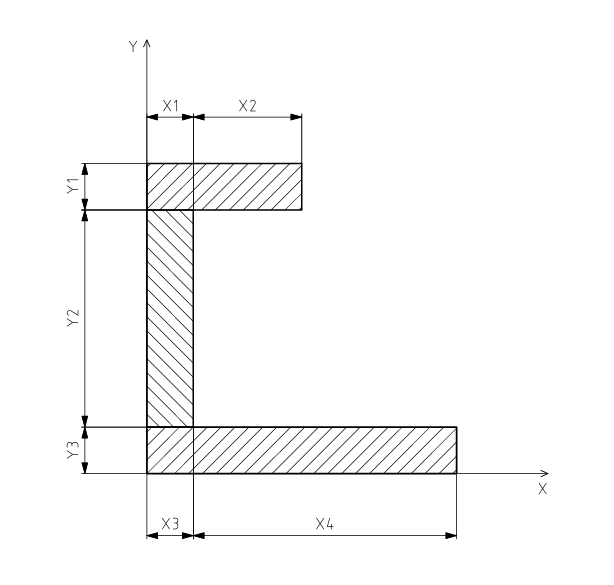
\includegraphics[width=\textwidth]{size.png}
        \caption{Průřez tělesa}
        \label{fig:my_picture}
    \end{minipage}
    \hfill % Adds flexible space between the two minipages
    % ---- Second minipage for the Table ----
    \begin{minipage}[c]{0.3\textwidth}
        \centering
        \captionof{table}{Rozměry průřezu}
        \label{tab:my_table}
        \begin{tabular}{lccccc}
\toprule
\textbf{Rozměr} & $\boldsymbol{l}$ [mm] & $\boldsymbol{\nu}$ [-]  \\
\midrule
X1  & 30 & 0,2  \\
X2  & 70 & 0,2  \\
X3  & 30 & 0,2  \\
X4  & 170 & 0,2 \\
Y1  & 30 & 0,2  \\
Y2  & 140 & 0,2  \\
Y3  & 30 & 0,2  \\
\bottomrule
\end{tabular}
    \end{minipage}
    
\end{figure}

 \newpage

\subsection{Řešení}

\subsubsection{Osové kvadratické momenty}
Pro osový kvadratický moment obdélníku platí: 
\begin{equation}
    I =  \frac{b_i}{3}  \cdot (h_i^3-L^3)  
\end{equation}
kde b odpovídá délce strany rovnoběžné s osou, h odpovídá délce strany kolmé na osu a L odpovídá vzdálenosti obdélníku od osy. 

Osový kvadratický moment tělesa, složeného z více obdélníků, pak odpovídá součtu jejich osových kvadratických momentů.

Na základě vzorce 1 lze vyjádřit kvadratický moment pro jednotlivé obdélníky k ose X jako:
\\ 
 \\ 
Horní pásnice:
\begin{equation}
    I_{x3} =  \frac{1}{3}  \cdot(X1 + X2) \cdot ((Y1 + Y2 + Y3)^3 - (Y2 + Y3)^3)
\end{equation}
Stojina:
\begin{equation}
    I_{x2} =  \frac{1}{3}  \cdot X1 \cdot ((Y3 + Y2)^3 - Y3^3) 
\end{equation}
Dolní pásnice:
\begin{equation}
    I_{x1} =  \frac{1}{3}  \cdot (X3 + X4) \cdot Y3^3 
\end{equation}
Celkový osový kvadratický moment:
\begin{equation}
    I_x =  \sum_{i=1}^{3}  I_{xi}
\end{equation}
 
a k ose Y jako:
\\ 
 \\ 
\noindent Horní pásnice:
\begin{equation}
    I_{y1} =  \frac{1}{3}  \cdot Y1 \cdot  (X1 + X2)^3  
\end{equation}
Stojina:
\begin{equation}
    I_{y2} =  \frac{1}{3}  \cdot Y2 \cdot X1^3
\end{equation}
Dolní pásnice:
\begin{equation}
    I_{y3} =  \frac{1}{3}  \cdot Y3 \cdot (X3 + X4)^3
\end{equation}
Celkový osový kvadratický moment:
\begin{equation}
    I_y =  \sum_{i=1}^{3} I_{yi}
\end{equation}

\subsubsection{ Zpracování metodou Monte Carlo}

Rozměrové veličiny  jsou popsány normálním rozdělením s~$\mathrm{\nu} = 0{,}2$. Pro potřeby numerického řešení metodou Monte Carlo byly v programu Matlab R2024B vygenerovány statistické soubory o počtu prvků $N = 1\E{8}$ pro každou z nich. 
Na jejich základě byly vypočítány střední hodnoty kvadratických osových momentů k oběma osám, jejich směrodatné odchylky a variační koeficienty. Ty zobrazuje tabulka 2.


\begin{table}[H]
\centering
\caption{Statistické charakteristiky osových kvadratických momentů }
\begin{tabular}{lcccc}
\toprule
\textbf{Veličina} & $\boldsymbol{\mu}$ [$\E{6}$ mm$^4$] & $\boldsymbol{\sigma}$ [$\E{6}$ mm$^4$] & $\boldsymbol{\nu}$ [-] \\
\midrule
$I_{x}$ & 161{,}10 & 68{,}21 & 0{,}423  \\
$I_{y}$ & 99{,}26 & 48{,}34 & 0{,}487  \\
\bottomrule
\end{tabular}
\end{table}

\noindent Variační koeficienty výstupu ($0{,}42$--$0{,}49$) jsou oproti vstupu ($0{,}2$) více než dvojnásobné, to je dáno jejich závislostí na rozměrech ve třetí mocnině (zesílení nejistoty). 

Histogramy pro oba statistické soubory osových kvadratických momentů zobrazuje obrázek 2. Důvodem pro jejich asymetrii je opět třetí mocnina vstupů.


\begin{figure}[htbp]
    \centering
    
    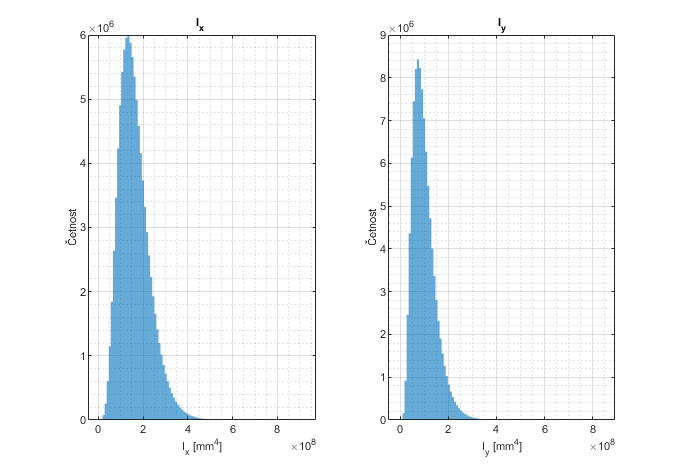
\includegraphics[width=0.8\textwidth]{histo.png} 
    \caption{Histogramy osových kvadratických momentů z Monte Carlo}
    \label{fig:single_picture}
\end{figure}
Srovnání obou statistických souborů normalizovaných s pomocí hustoty pravděpodnosti je vykresleno na obrázku 3.
\begin{figure}[htbp]
    \centering
    
    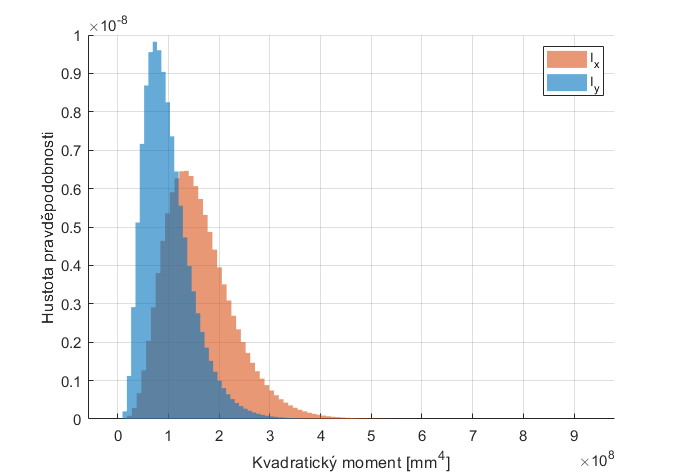
\includegraphics[width=0.7\textwidth]{hustoty.png} 
    \caption{Srovnání hustot pravděpodobnosti osových kvadratických momentů}
    \label{fig:single_picture}
\end{figure}

\clearpage

\section{Příklad 3E -- Pravděpodobnost bezporuchového provozu}



V klínových řemenech byla zjištěna následující provozní napětí $\sigma_p$ v MPa:

\[
\sigma_p =
\{223;\ 116;\ 158{,}5;\ 199;\ 136{,}5;\ 169{,}5;\ 267{,}5;\ 127;\ 184;\ 151\}
\]


\noindent
Dále byly zjištěny následující hodnoty meze pevnosti $R_m$ v MPa:

\[
R_m =
\{211;\ 269{,}5;\ 192;\ 301{,}5;\ 220{,}5;\ 243{,}5;\ 182{,}5;\ 257;\ 234;\ 199{,}5;\ 216;\ 205\}
\]

Cílem výpočtu je stanovit pravděpodobnost bezporuchového provozu ve tvaru:

\begin{equation}
P_{\text{bezp.}} = P(R_m > \sigma_p)
\label{eq:pravd}
\end{equation}

\subsection*{Předpoklad výpočtu}

Obě veličiny byly uvažovány jako náhodné s normálním rozdělením:

\begin{equation}
\sigma_p \sim \mathcal{N}(\mu_{\sigma}, s_{\sigma}), \qquad
R_m \sim \mathcal{N}(\mu_R, s_R)
\label{eq:normalita}
\end{equation}


\noindent
Z dat byly stanoveny statistické charakteristiky:

\[
\mu_{\sigma} = 173{,}20\ \text{MPa}, \quad
s_{\sigma} = 46{,}70\ \text{MPa}
\]

\[
\mu_R = 227{,}67\ \text{MPa}, \quad
s_R = 34{,}95\ \text{MPa}
\]

\subsection*{Kontrola normality}

Pro ověření předpokladu normálního rozdělení byla zvolena hladina významnosti:
\[
\alpha = 0{,}05
\]
Při této hladině významnosti se rozhoduje o zamítnutí nulové hypotézy na základě~p-~hodnoty.

Dále byl použit Lillieforsův test, který je modifikací Kolmogorov--Smirnovova testu a je vhodný v případech, kdy parametry normálního rozdělení nejsou předem známy, ale jsou odhadovány z dat. Tento test je v prostředí MATLAB implementován přímo pomocí funkce \texttt{lillietest}, která umožňuje automatický výpočet testovací statistiky i p-hodnoty.

Normalita dat byla současně ověřena i vizuálně pomocí Q-Q diagramu (obr.~\ref{fig:qq_plot}).

\begin{figure}[H]
    \centering
    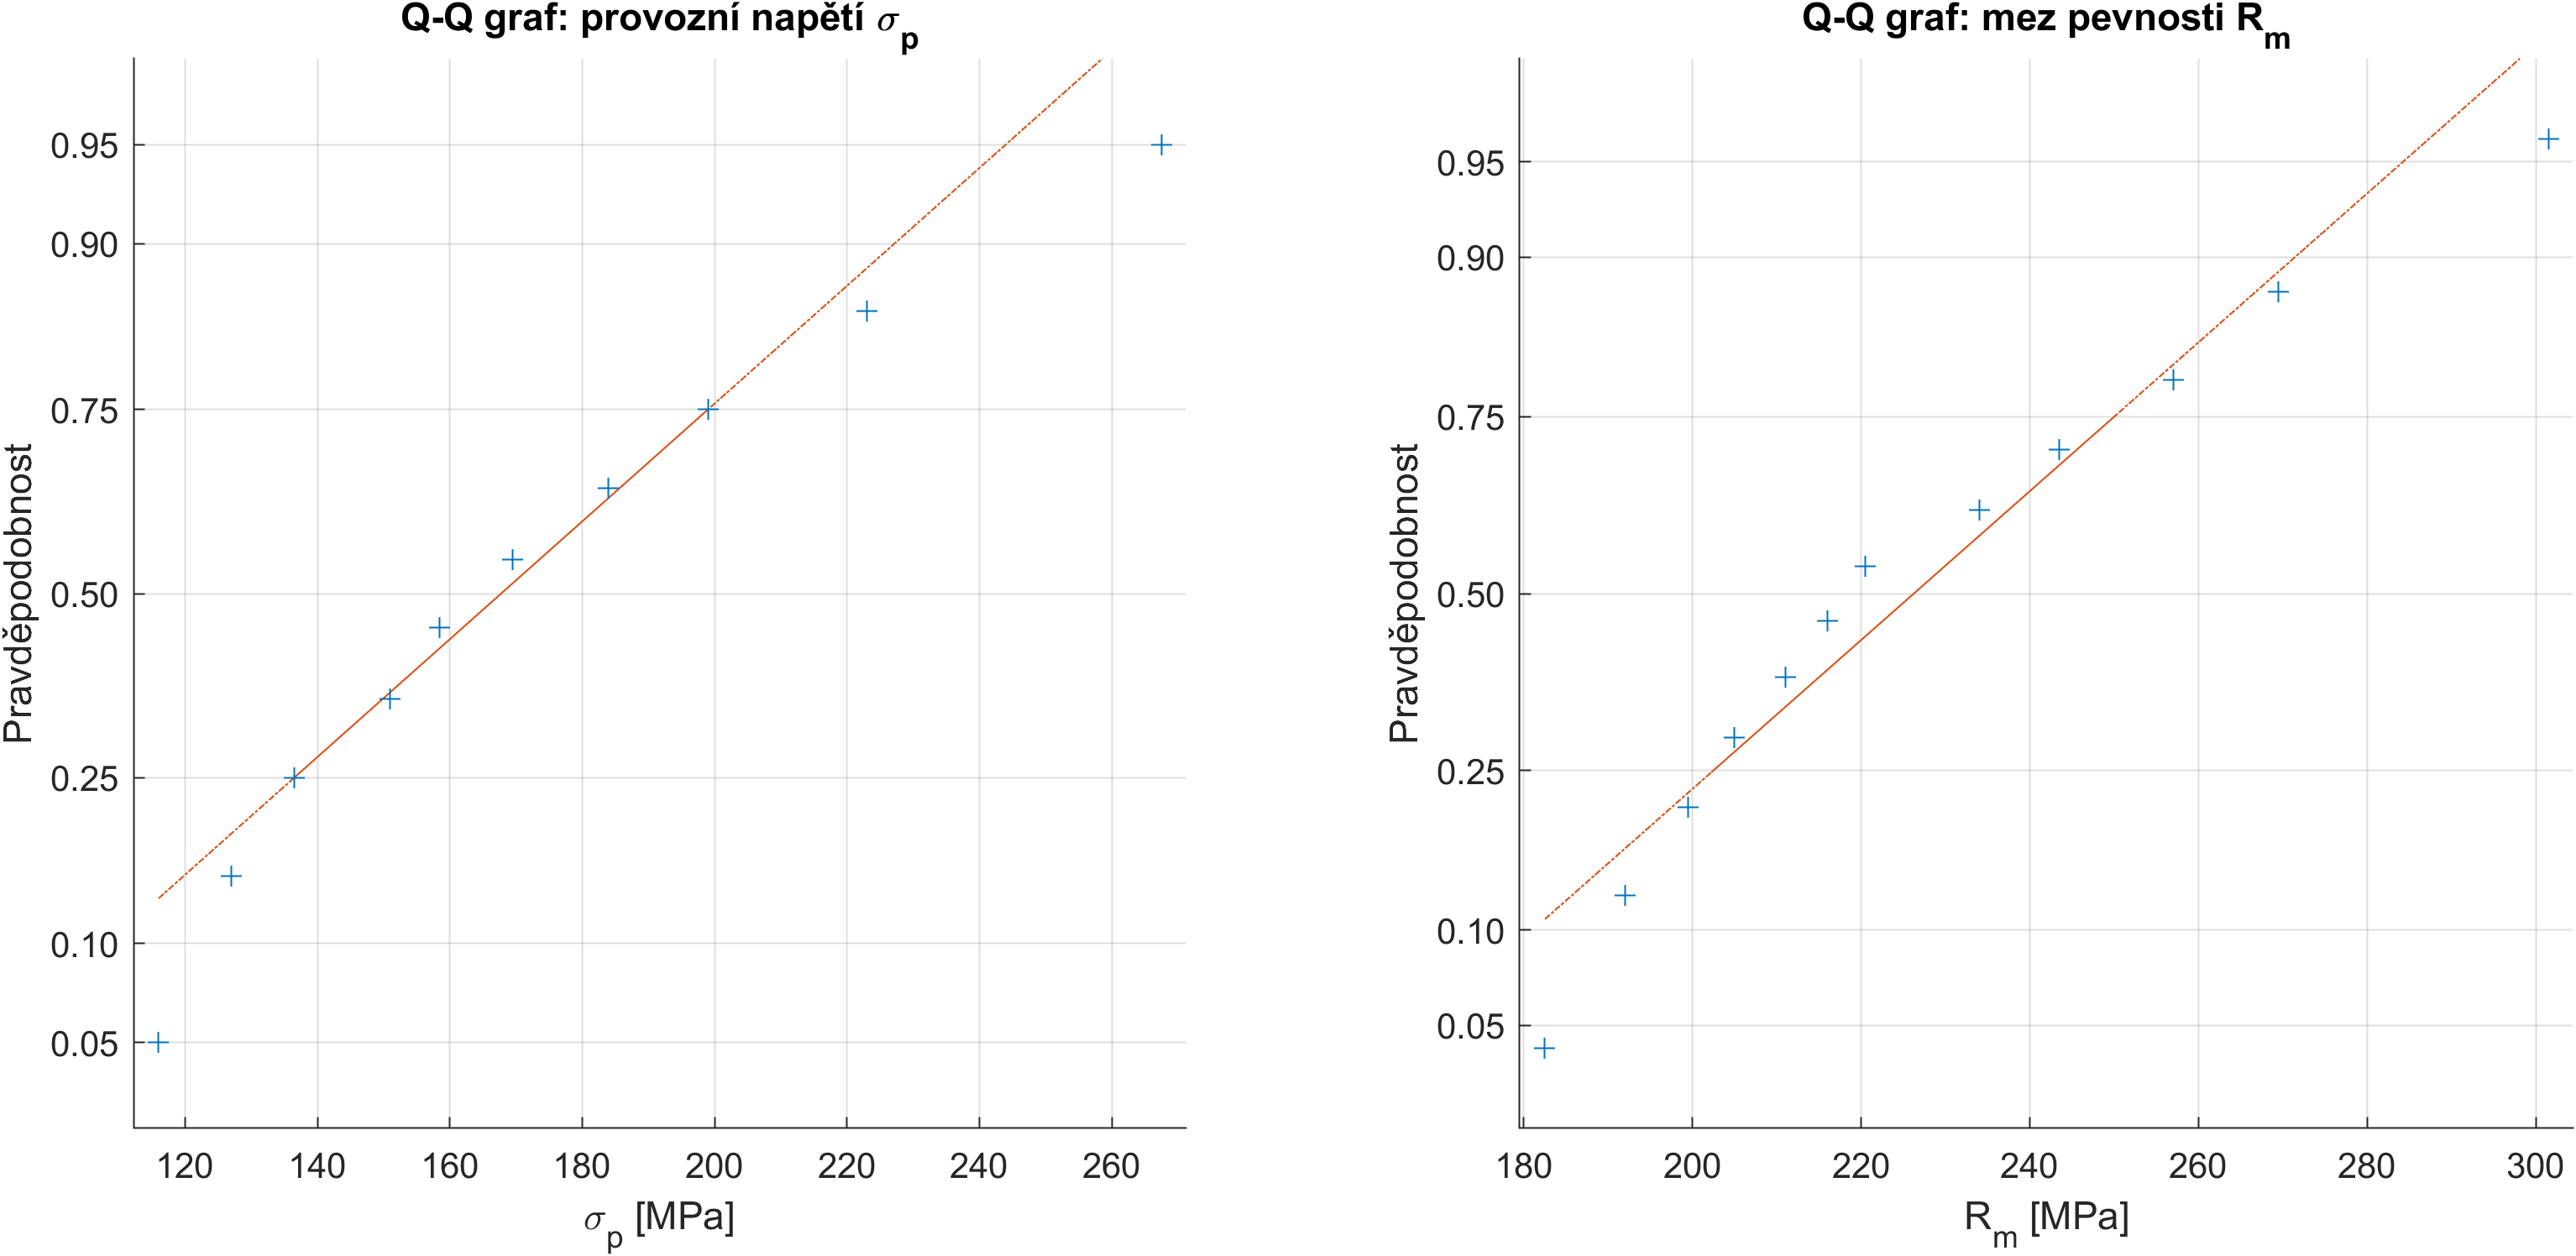
\includegraphics[width=0.95\textwidth]{qq_grafy.png}
    \caption{Q-Q diagram pro provozní napětí $\sigma_p$ a mez pevnosti $R_m$}
    \label{fig:qq_plot}
\end{figure}

Výsledky testu:

\[
p_{\sigma_p} = 0{,}5000, \qquad p_{R_m} = 0{,}4792
\]

\noindent
Protože v obou případech platí $p > \alpha = 0{,}05$, nelze zamítnout nulovou hypotézu o normálním rozdělení.  
Předpoklad uvedený ve vztahu~(\ref{eq:normalita}) je tedy pro další výpočet přijatelný.

\subsection*{Výpočet indexu spolehlivosti}

Zavedeme rozdílovou veličinu:

\begin{equation}
Z = R_m - \sigma_p
\label{eq:Z}
\end{equation}

\noindent
Bezporuchový provoz nastává, pokud $Z > 0$. Index spolehlivosti je definován jako:

\begin{equation}
\beta =
\frac{\mu_R - \mu_{\sigma}}
{\sqrt{s_R^2 + s_{\sigma}^2}}
\label{eq:beta}
\end{equation}

Po dosazení:

\[
\beta =
\frac{227{,}67 - 173{,}20}
{\sqrt{34{,}95^2 + 46{,}70^2}}
= 0{,}9337
\]

\subsection*{Výpočet pravděpodobnosti}

Hledaná pravděpodobnost ze vztahu~(\ref{eq:pravd}) se určí pomocí distribuční funkce normálního rozdělení:

\begin{equation}
P_{\text{bezp.}} = \Phi(\beta)
\label{eq:Phi}
\end{equation}

Po dosazení:

\[
P_{\text{bezp.}} = \Phi(0{,}9337) = 0{,}8248
\]

\[
P_{\text{bezp.}} = 82{,}48 \%
\]

\subsection*{Závěr}

Na základě provedeného výpočtu byla pravděpodobnost bezporuchového provozu stanovena jako:

\[
\boxed{P_{\text{bezp.}} = 0{,}8248 \approx 82{,}48\,\%}
\]

\noindent
Pravděpodobnost poruchy je:

\[
\boxed{P_{\text{por.}} = 0{,}1752 \approx 17{,}52\,\%}
\]

\noindent
Při uvažovaném normálním rozdělení veličin $\sigma_p$ a $R_m$ je tedy pravděpodobnost bezporuchového provozu přibližně $82{,}5\,\%$.


\clearpage

\input{4E/priklad_4E.tex}
\clearpage


%% ============================================================
%% PŘÍKLAD 5E
%% ============================================================
\section{Příklad 5E -- Časový průběh napětí ve vrubech}

\subsection{Zadání}

Rotační hřídel se dvěma zápichy, axiálně zatížená střídavou silou s~obdélníkovým časovým průběhem.

\textbf{Geometrie} (z~výkresu, celková délka $L_{\mathrm{tot}} = 820\unit{mm}$):
\begin{itemize}[nosep]
    \item Hlavní průměr $D = 50\unit{mm}$, průměr v~zápichu $d = 35\unit{mm}$
    \item Poloměr zápichu $r = 5\unit{mm}$, šířka zápichu $10\unit{mm}$
    \item Úseky: $200 + 10 + 400 + 10 + 200\unit{mm}$
    \item Síla působí v~$x_F = 500\unit{mm}$ od levého vetknutí
    \item Levý vrub: $x \in [200; 210]\unit{mm}$ (před silou)
    \item Pravý vrub: $x \in [610; 620]\unit{mm}$ (za silou)
\end{itemize}

\textbf{Uložení:}
\begin{itemize}[nosep]
    \item \textbf{Vlevo:} pevné vetknutí
    \item \textbf{Vpravo:} jednostranný kontakt s~tuhou stěnou ($\delta = 0$). Posuv do stěny nemožný, od stěny volný — pravá podpora přenáší pouze tlak.
\end{itemize}

\textbf{Zatížení:} obdélníková střídavá osová síla $F = \pm 1{,}4\cdot 10^5\unit{N}$, tolerance velikosti síly $+1000/-0\unit{N}$. Tolerance geometrie $\pm 0{,}5\unit{mm}$ na všech rozměrech.

\textbf{Cíl:} stanovit časový průběh lokálního napětí v~obou vrubech (statický výpočet, $K_t$).

\begin{figure}[H]
\centering
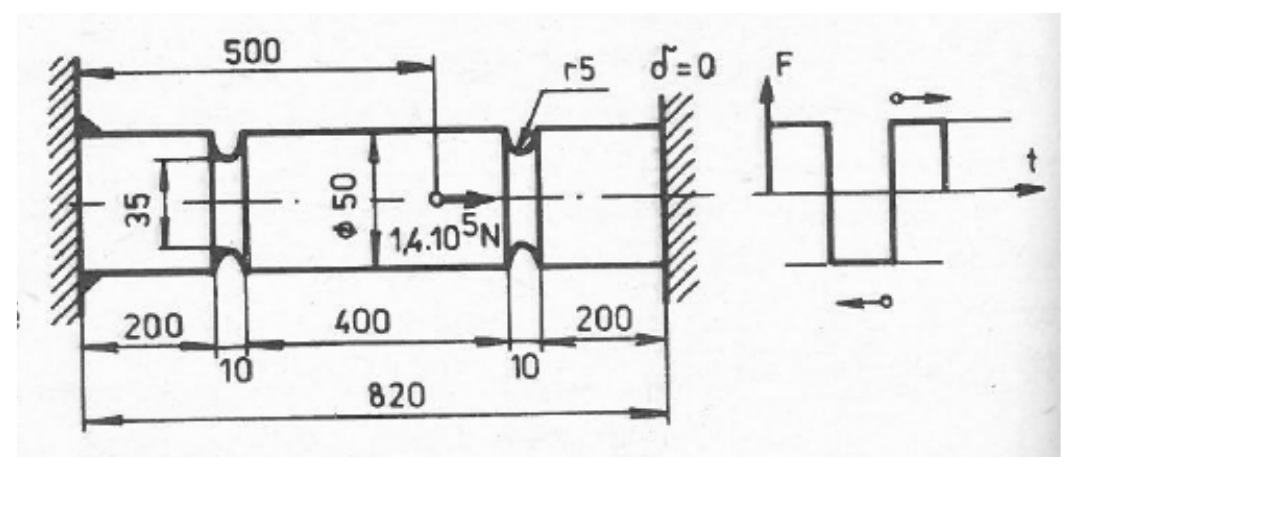
\includegraphics[width=0.85\textwidth]{priklad_5E_zadani.png}
\caption{Zadání: rotační hřídel se dvěma zápichy a~jednostranným kontaktem vpravo, F~$=\pm 1{,}4\E{5}\unit{N}$.}
\end{figure}

\subsection{Deterministické řešení}

\subsubsection{Stav A — staticky neurčitá úloha}

Konvence: tah $+x$ doprava. Označme $R_R$ reakci od pravé stěny (působí v~$-x$, tedy $R_R \le 0$).

Z pravé části hřídele plyne vnitřní osová síla:
\begin{align}
    N_{\mathrm{levá}}(x < x_F) &= F + R_R \\
    N_{\mathrm{pravá}}(x > x_F) &= R_R
\end{align}

\textbf{Podmínka kompatibility} (pravý konec se nepohne, $\Delta_{\mathrm{tot}} = 0$):
\begin{equation}
    N_{\mathrm{levá}} \cdot C_L + N_{\mathrm{pravá}} \cdot C_R = 0
\end{equation}
kde $C_L$, $C_R$ jsou osové poddajnosti levé a~pravé části (násobeno $E$):
\begin{align}
    A_D &= \frac{\pi D^2}{4} = 1963{,}5\unit{mm^2}, \quad A_d = \frac{\pi d^2}{4} = 962{,}1\unit{mm^2} \\
    C_L &= \frac{490}{A_D} + \frac{10}{A_d} = 0{,}24955 + 0{,}01039 = 0{,}25995\unit{mm/mm^2} \\
    C_R &= \frac{310}{A_D} + \frac{10}{A_d} = 0{,}15788 + 0{,}01039 = 0{,}16827\unit{mm/mm^2}
\end{align}

Řešení:
\begin{align}
    R_R &= -F \cdot \frac{C_L}{C_L + C_R} = -140000 \cdot \frac{0{,}25995}{0{,}42822} = -84\,985\unit{N} \\
    N_{\mathrm{levá}}^A &= F + R_R = +55\,015\unit{N} \quad \\
    N_{\mathrm{pravá}}^A &= R_R = -84\,985\unit{N} \quad
\end{align}

\subsubsection{Stav B — staticky určitá úloha}

Pravý konec se odlepí, $R_R = 0$. Z~rovnováhy:
\begin{align}
    N_{\mathrm{levá}}^B &= F + 0 = -140\,000\unit{N} \quad \\
    N_{\mathrm{pravá}}^B &= 0
\end{align}

\subsubsection{Součinitel koncentrace napětí}

Geometrické poměry pro Petersonův graf (kruhový hřídel s~U-vrubem, axiální tah):
\begin{equation}
    \frac{D}{d} = 1{,}429, \qquad \frac{r}{d} = 0{,}143 \quad\Rightarrow\quad \boxed{K_t \approx 2{,}10}
\end{equation}

\begin{figure}[H]
\centering
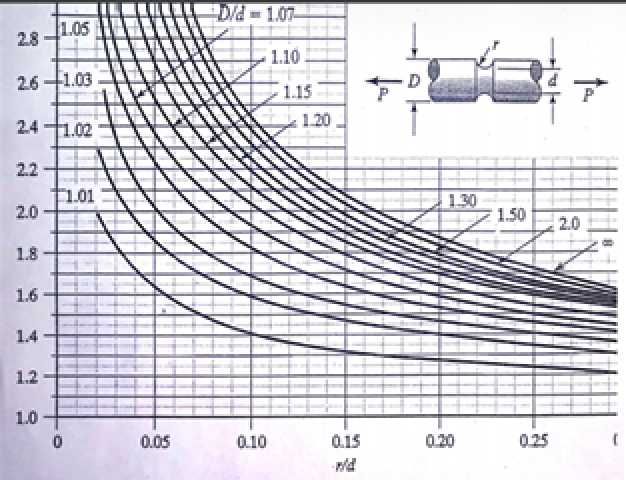
\includegraphics[width=0.5\textwidth]{peterson1.png}
\caption{Petersonův graf pro kruhový hřídel s U vrubem při axiálním tahu}
\end{figure}

(Neuberova aproximace $K_t = 1 + 2\sqrt{t/r} = 3{,}449$ je horní konzervativní mez; Petersonův graf preferován jako přesnější.)

\subsubsection{Lokální napětí ve vrubech}

\textbf{Levý vrub} (v~levé části, působí oba stavy):
\begin{align}
    \sigma_{\mathrm{L}}^A &= K_t \cdot \frac{N_{\mathrm{levá}}^A}{A_d} = 2{,}10 \cdot \frac{55\,015}{962{,}1} = \boxed{+120{,}1\unit{MPa}} \\
    \sigma_{\mathrm{L}}^B &= K_t \cdot \frac{N_{\mathrm{levá}}^B}{A_d} = 2{,}10 \cdot \frac{-140\,000}{962{,}1} = \boxed{-305{,}6\unit{MPa}}
\end{align}

\textbf{Pravý vrub} (v~pravé části, působí jen Stav~A):
\begin{align}
    \sigma_{\mathrm{R}}^A &= K_t \cdot \frac{N_{\mathrm{pravá}}^A}{A_d} = 2{,}10 \cdot \frac{-84\,985}{962{,}1} = \boxed{-185{,}5\unit{MPa}} \\
    \sigma_{\mathrm{R}}^B &= 0\unit{MPa}
\end{align}

\subsection{Časový průběh napětí}

Síla $F(t)$ obdélníkově střídá hodnoty $+140\unit{kN}$ a~$-140\unit{kN}$. Statický výpočet $\Rightarrow$ napětí mezi dvěma diskrétními hodnotami:

\begin{center}
\begin{tabular}{lcccccc}
\toprule
\textbf{Vrub} & $\sigma_{\max}$ & $\sigma_{\min}$ & $\sigma_a$ & $\sigma_m$ & $R = \sigma_{\min}/\sigma_{\max}$ & \textbf{Charakter cyklu} \\
\midrule
Levý  & $+120{,}1$ & $-305{,}6$ & $212{,}8$ & $-92{,}8$ & $-2{,}55$ & asymetrický střídavý \\
Pravý & $0$        & $-185{,}5$ & $92{,}8$  & $-92{,}8$ & $\pm\infty$ & míjivý tlak (0 $\leftrightarrow$ tlak) \\
\bottomrule
\end{tabular}
\end{center}

\subsection{Stochastická analýza}

Rozměry s~tolerancí $\pm 0{,}5\unit{mm}$: $\sigma_{\mathrm{dim}} = 0{,}5/3 \approx 0{,}167\unit{mm}$ (pravidlo $3\sigma$, normální rozdělení). Síla $F \sim \mathcal{U}(140\,000;\,141\,000)\unit{N}$ (uniformní, dle tolerance $+1000/-0$). Náhodné: $D, d, r$, všech 5 délek úseků, poloha síly $x_F$, velikost síly $F$.

\begin{table}[H]
\centering
\caption{Statistiky napětí v~obou vrubech ($N = 100\,000$)}
\begin{tabular}{lccccc}
\toprule
\textbf{Veličina} & $\boldsymbol{\mu}$ & $\boldsymbol{\sigma}$ & \textbf{CoV} & \textbf{95\% CI} \\
\midrule
$\sigma_{\mathrm{L,max}}$ [MPa] & $+120{,}54$ & $1{,}91$ & $0{,}016$ & $[+116{,}85;\; +124{,}33]$ \\
$\sigma_{\mathrm{L,min}}$ [MPa] & $-306{,}74$ & $4{,}80$ & $0{,}016$ & $[-316{,}32;\; -297{,}44]$ \\
$\sigma_{\mathrm{L},a}$    [MPa] & $+213{,}64$ & $3{,}35$ & $0{,}016$ & $[+207{,}15;\; +220{,}32]$ \\
$\sigma_{\mathrm{R,min}}$ [MPa] & $-186{,}20$ & $2{,}91$ & $0{,}016$ & $[-192{,}00;\; -180{,}59]$ \\
$\sigma_{\mathrm{R},a}$    [MPa] & $+93{,}10$  & $1{,}45$ & $0{,}016$ & $[+90{,}29;\; +96{,}00]$ \\
$K_t$ [-] & $2{,}100$ & $0{,}020$ & $0{,}010$ & $[2{,}06;\; 2{,}14]$ \\
\bottomrule
\end{tabular}
\end{table}

Variabilita napětí $\mathrm{CoV} \approx 1{,}6\%$ — nízká, dominuje rozptyl $A_d$ (kvadratická závislost na $d$) a~$K_t$ (citlivost na $r$). Rozptyl síly přispívá řádově $0{,}2\%$ (úzká tolerance).

\begin{figure}[H]
\centering
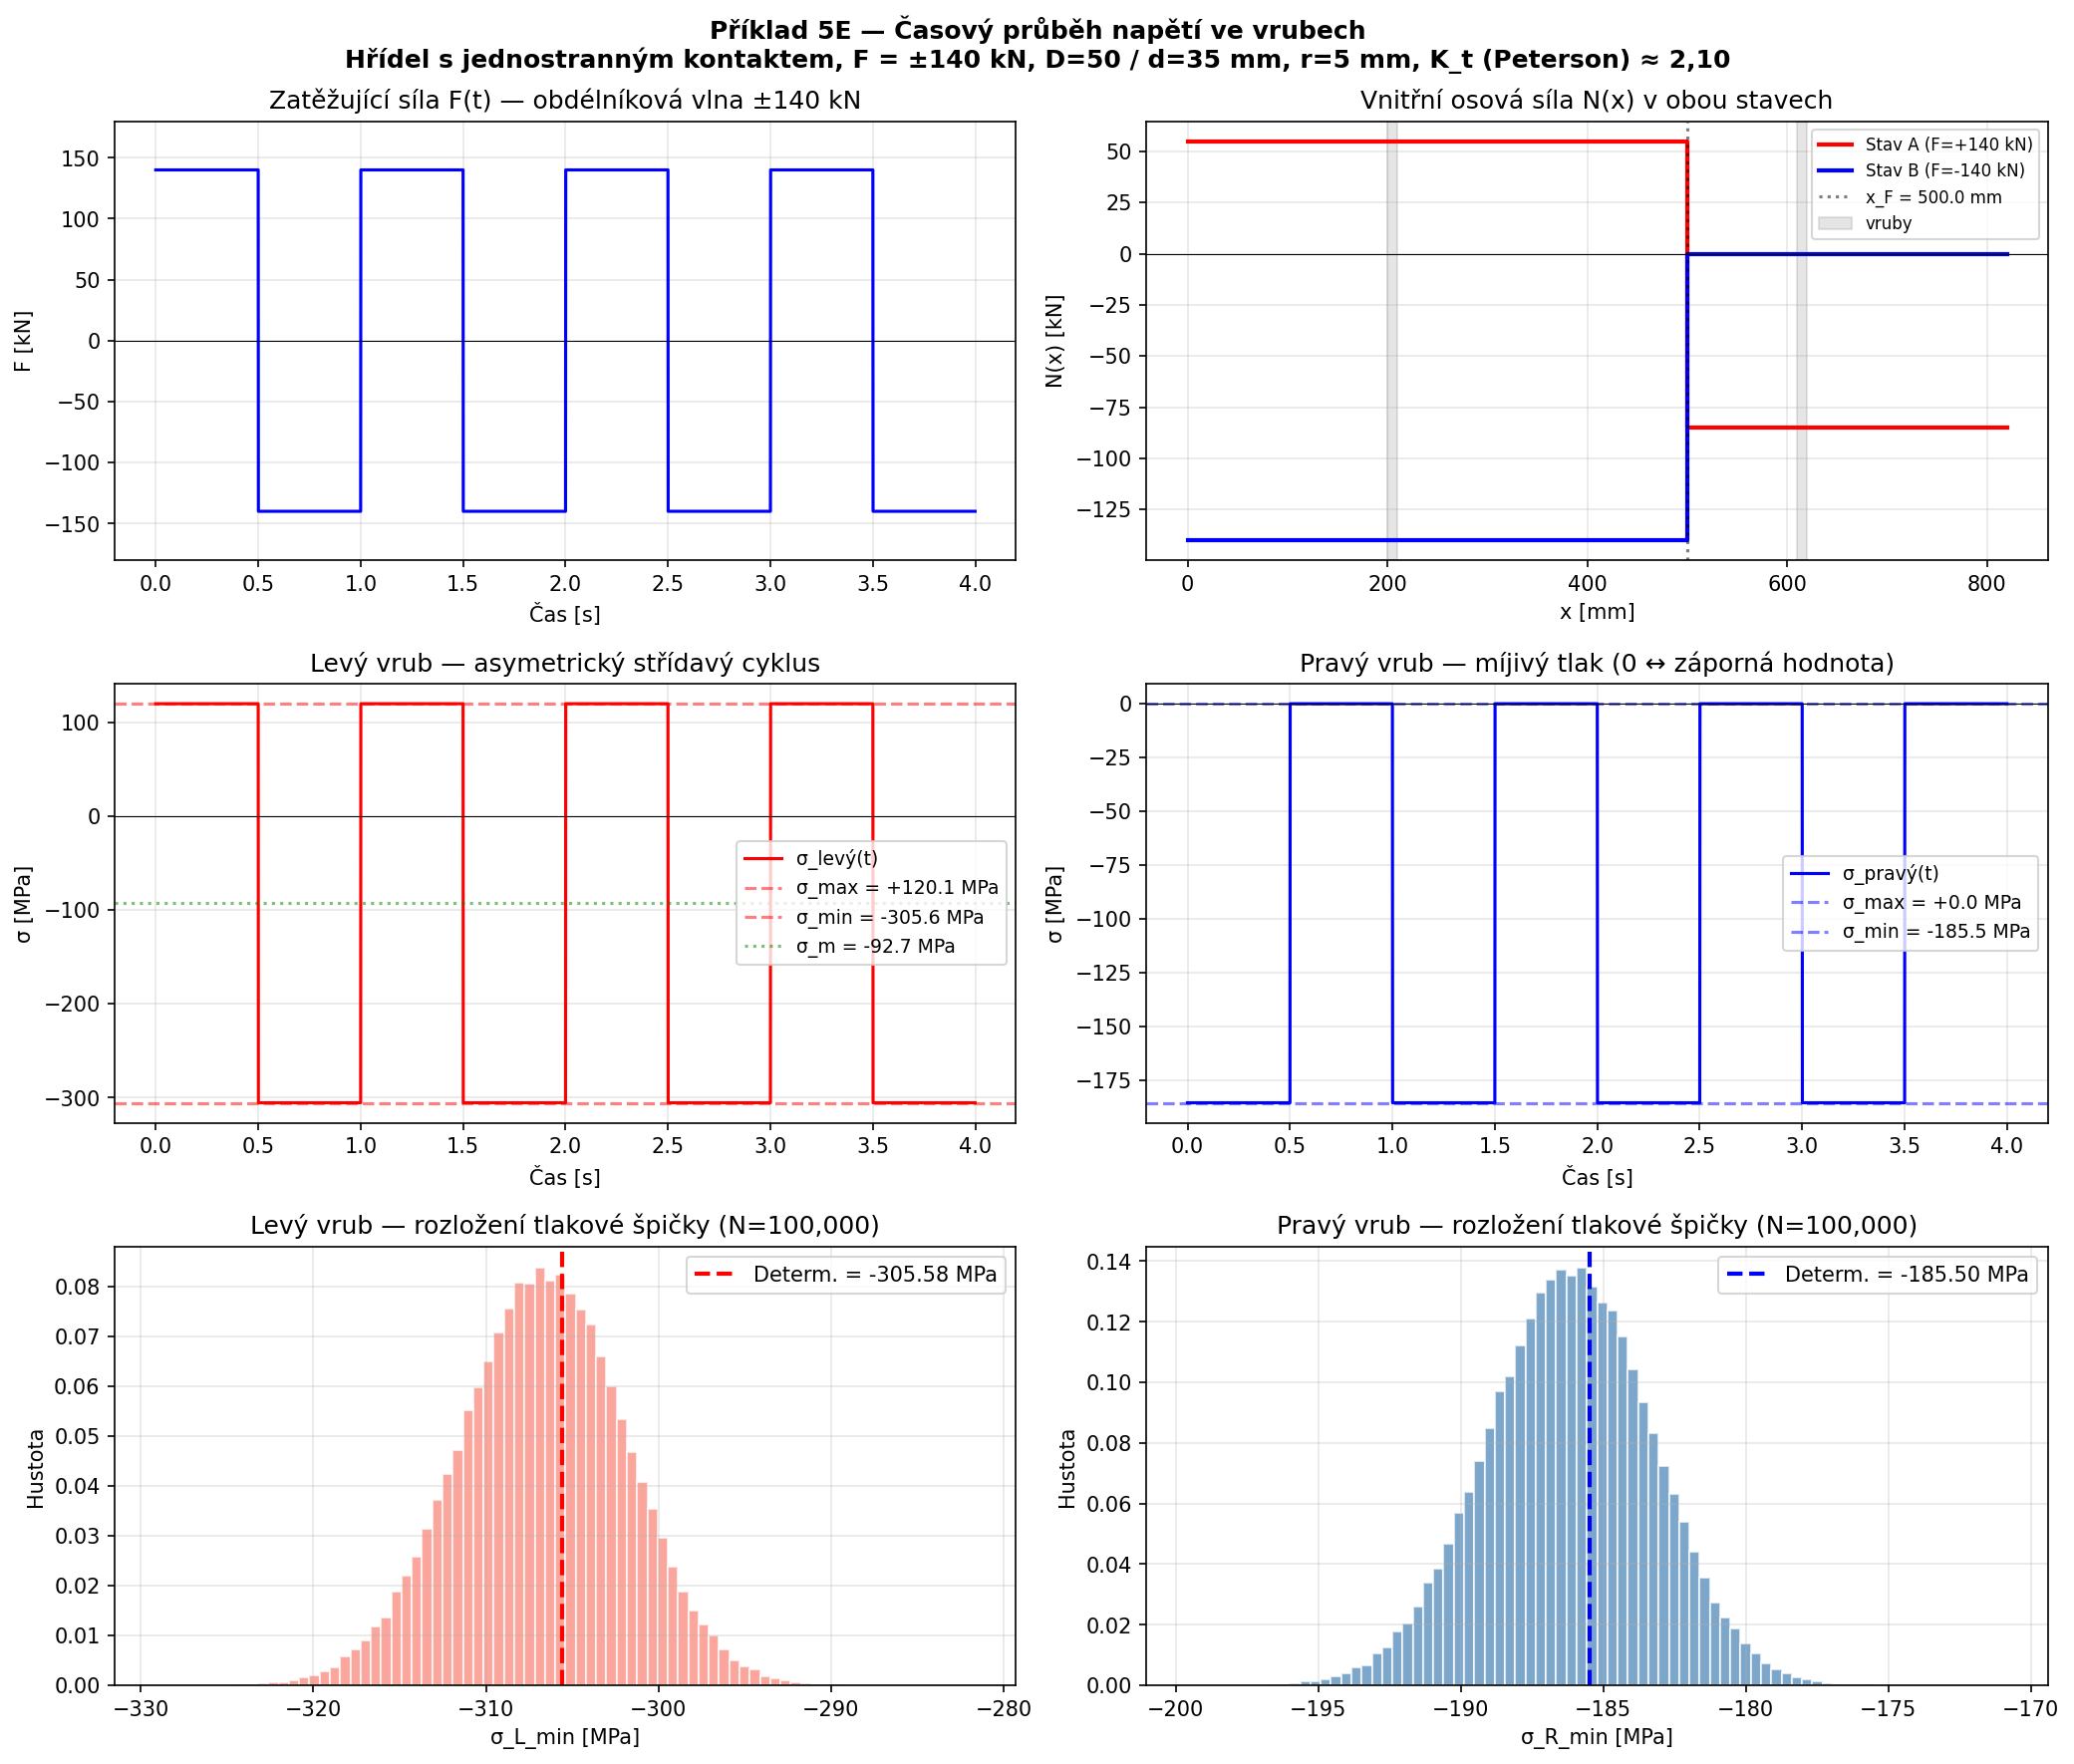
\includegraphics[width=\textwidth]{priklad_5E_vysledky.png}
\caption{Příklad 5E -- Časový průběh síly a~napětí, stochastická analýza}
\label{fig:5E}
\end{figure}

\begin{figure}[H]
\centering
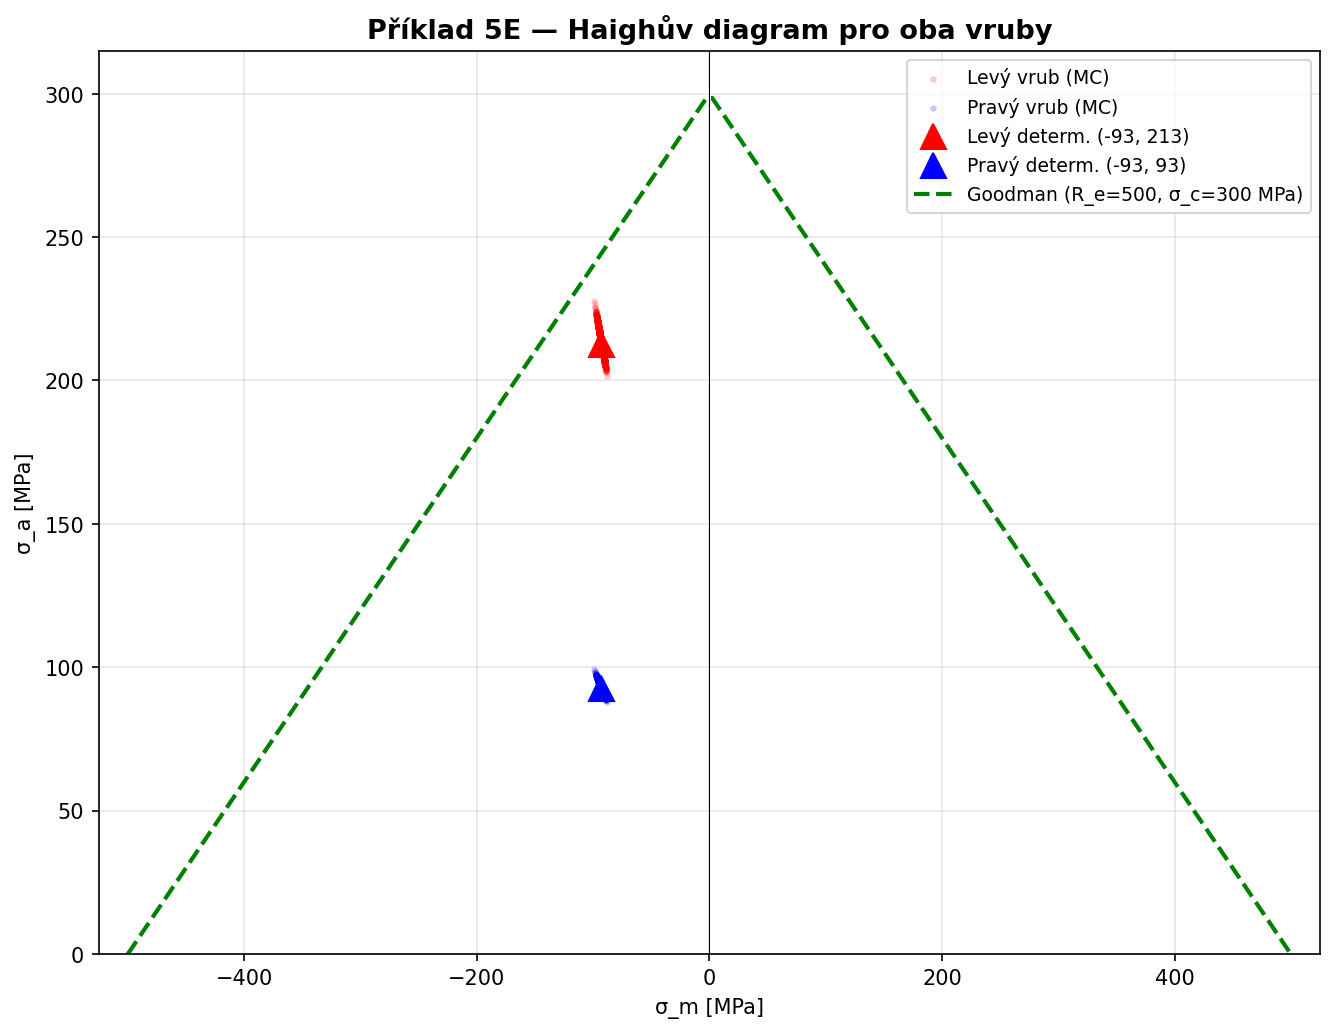
\includegraphics[width=0.5\textwidth]{priklad_5E_haigh.png}
\caption{Příklad 5E -- Haighův diagram ($\sigma_a$ vs $\sigma_m$) s~Goodmanovou přímkou}
\label{fig:5E_haigh}
\end{figure}



\end{document}
